\documentclass[12pt]{article}					% Začátek dokumentu
\usepackage{../../MFFStyle}					    % Import stylu



\begin{document}

% 07. 10. 2021
\section{Návrh}
\begin{poznamka}[Co je potřeba]
	Typy, vztahy (arita, kardinalita), vlastnosti (kardinalita).
\end{poznamka}

\begin{center}
	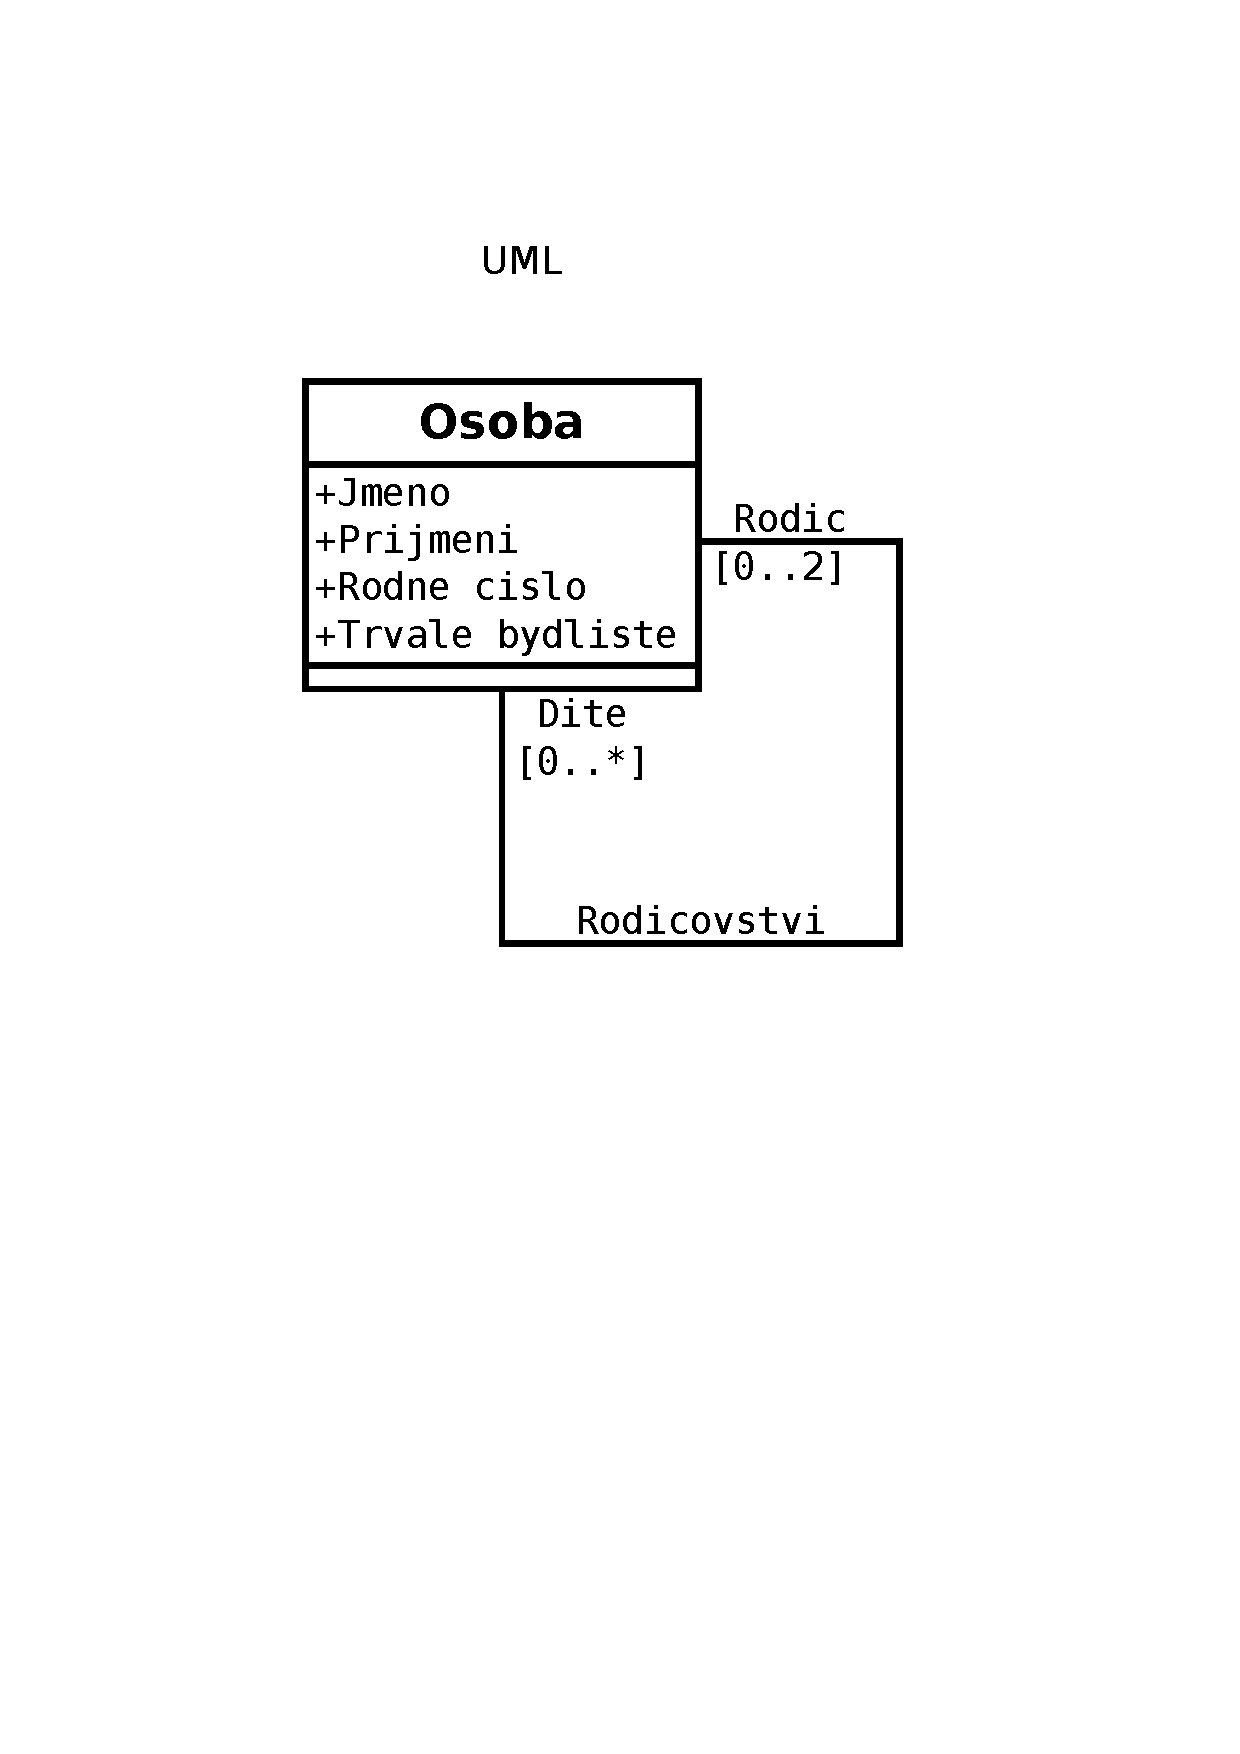
\includegraphics[width=0.3\textwidth]{UMLvsER.pdf}
	\includegraphics[width=0.3\textwidth, page=2]{UMLvsER.pdf}
\end{center}

\begin{definice}[UML]
	Zaznamenává vztahy jako hrany, kardinalitu konce píše k tomu konci. Tj. má u sebe napsaný název „orientovaného“ vztahu a jeho kardinalitu (např. rodič, [0, 2]). Atributy (vlastnosti) reprezentuje přímo v objektu. Pokud chci přidat atribut vlastnosti, musím vytvořit objekt, který se k ní váže. Kardinalita atributů se píše k němu do objektu.
\end{definice}

\begin{definice}[ER]
	Reprezentuje vztahy jako další objekty, kardinalitu píše na výstupní hranu. Tj. má u sebe napsaný název „orientovaného vztahu“ a kardinalitu opačného vztahu (např. dítě [0, 2]). Atributy reprezentuje jako další objekty. Pokud chci přidat atribut vlastnosti, tak to dělám stejně jako u objektu. Kardinalita atributů se píše k hraně.
\end{definice}


\end{document}
